\chapter{Tinjauan Pustaka}
\label{chap:tinjauan-pustaka}

\section{Hasil Penelitian Terdahulu}

Penelitian ini merujuk pada berbagai studi ilmiah dan penelitian terdahulu yang membahas sistem penyerbukan kelapa sawit, perilaku \emph{Elaeidobius kamerunicus}, serta pemanfaatan
teknologi drone dan sensor cerdas dalam pertanian presisi. Literatur yang dikumpulkan
mencakup penelitian tentang kematangan bunga sawit berdasarkan citra, desain mekanisme
penyerbukan buatan, hingga navigasi otonom berbasis UAV. Seluruh referensi tersebut
digunakan sebagai landasan dalam merancang metode deteksi kesiapan penyerbukan, sistem
mekanik penyerbuk pada drone, dan pergerakan otonom UAV pada penelitian ini. Tabel 2.1
menyajikan ringkasan penelitian terdahulu yang menjadi acuan dalam pengembangan proyek
ini.

\begin{longtable}{|c|p{4cm}|p{9cm}|}
  \caption{Penelitian Terdahulu}\label{tab:penelitian-terdahulu} \\
  \hline
  \textbf{No} & \textbf{Penelitian} & \textbf{Pembahasan} \\
  \hline
  \endfirsthead
  
  \multicolumn{3}{c}{\tablename\ \thetable\ -- \textit{Lanjutan dari halaman sebelumnya}} \\
  \hline
  \textbf{No} & \textbf{Penelitian} & \textbf{Pembahasan} \\
  \hline
  \endhead
  
  \hline
  \endfoot
  
  \hline
  \endlastfoot
  
  1 & Oil palm trees detection and counting on Microsoft Bing Maps Very High
Resolution (VHR) satellite imagery and Unmanned Aerial Vehicles (UAV) data
using image processing thresholding approach \parencite{putra2022oil} &
  Mengembangkan metode deteksi dan penghitungan pohon kelapa sawit menggunakan citra satelit VHR dan data UAV dengan pendekatan \emph{image processing} berbasis \emph{thresholding}; menghasilkan akurasi deteksi di atas 80\%, namun belum mendukung deteksi masa polinasi maupun \emph{robot-assisted pollination}. \\
  \hline

  2 & Multi-class oil palm trees condition detection from UAV images using Faster R-CNN with EfficientNetV2 \parencite{haq2024multiclass} &
  Mengusulkan sistem deteksi kondisi pohon kelapa sawit multi-kelas (\emph{dead, healthy, mismanaged, smallish, yellowish}) dari citra UAV menggunakan Faster R-CNN dengan \emph{backbone} EfficientNetV2; mencapai \emph{precision} 0,867, \emph{recall} 0,770, dan F1-score 0,805, berfokus pada kondisi tanaman, bukan penyerbukan. \\
  \hline

  3 & Implementasi CNN Dalam Mengidentifikasi Kematangan Cabai Berdasarkan Warna \parencite{ristiana2024implementasi} &
  Menerapkan CNN untuk mengidentifikasi kematangan cabai berdasarkan warna, menunjukkan bahwa CNN efektif untuk mengidentifikasi secara otomatis dan sistem mencapai akurasi 100\% dalam mengidentifikasi kematangan cabai. \\
  \hline

  4 & AI-Enabled Drones Detection for Precision Palm Pollination \parencite{alraeesi2024aienabled} &
  Menjelaskan penggunaan YOLO-small untuk membantu penyerbukan pohon kurma secara \emph{real-time} dalam polinasi berbasis \emph{drone}, didapatkan hasil mAP@0.5 sebesar 0.875 dan mengklaim reduksi biaya tenaga kerja ~80\%. \\
  \hline

  5 & An Autonomous Dual-Fan Pollination Device: Mathematical Modeling, Trajectory Optimization, and Distribution Analysis for Enhanced Crop Yield \parencite{gandhi2025autonomous} &
  Memperkenalkan perangkat penyerbukan buatan yang mampu mengumpulkan dan menyebarkan \emph{pollen} secara otomatis menggunakan corong cetak 3D, kipas hisap, sikat penyerbuk, dan kipas peniup. Pengujian menggunakan simulasi \emph{pollen} menunjukkan peningkatan tingkat keberhasilan dari 61\% menjadi 79\%, serta distribusi \emph{pollen} berbentuk kerucut yang dapat dioptimalkan hingga mencapai tingkat penyebaran 93--100\%. \\
  \hline

\end{longtable}

\section{Dasar Teori}

\subsection{Polinasi Kelapa Sawit}
\label{sec:polinasi-kelapa-sawit}

Polinasi atau penyerbukan pada Kelapa Sawit (\emph{Elaeis guineensis}) merupakan salah satu tahap penting dalam produktivitas kelapa sawit. Pada kelapa sawit, terdapat perbedaan masa \emph{anthesis} antara bunga jantan dan betina. Pada bunga jantan, masa \emph{anthesis} berlangsung selama 4-5 hari, sedangkan pada bunga betina berlangsung selama kurang lebih 2 hari.

\begin{figure}[H]
  \centering
  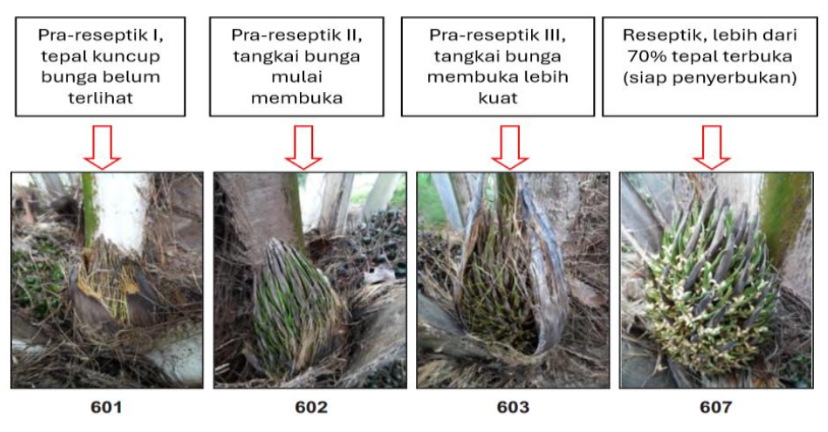
\includegraphics[width=0.6\textwidth]{gambar/polinasi.png}
  \caption{Perkembangan Kematangan Bunga Betina Kelapa Sawit \parencite{sujadi2021tahap}.}
  \label{fig:polinasi-kelapa-sawit}
\end{figure}

Pada masa \emph{anthesis}, terdapat ciri yang bisa dilihat secara langsung. Pada bunga jantan, terlihat \emph{pollen} berwarna kuning muda dan berukuran kecil yang mulai mekar dari bagian pangkal ke bagian ujung tandan bunga. Sedangkan untuk bunga betina, tampak mekar sempurna yang siap diserbuki, memiliki 3 cuping berambut, berbentuk menyerupai bulan sabit. Bunga sawit baik jantan maupun betina keduanya menghasilkan bau seperti bau adas. Bau khas ini yang dapat mengundang serangga polinator yang dapat menyebabkan terjadinya penyerbukan secara alami. Polinasi terjadi secara alami dengan bantuan serangga polinator yang efektivitasnya dipengaruhi oleh iklim mikro seperti suhu, kelembapan udara, dan kecepatan angin \parencite{sujadi2021tahap}.

\subsection{\emph{Convolutional Neural Network}}
\label{sec:cnn}

\emph{Convolutional Neural Network} (CNN) termasuk dalam kategori \emph{deep learning} dan sering digunakan dalam pemrosesan data gambar. CNN terinspirasi oleh proses-proses biologi dimana pola konektivitas antar neuron menyerupai \emph{cortex} pada binatang. Ide awal dari pengembangan \emph{deep learning}, yaitu memperjelas apa yang sebenarnya terjadi pada lapisan tersembunyi (\emph{hidden layer}) di dalam sebuah jaringan syaraf tiruan. Di dalam CNN terdapat empat lapisan utama antara lain lapisan konvolusi, lapisan aktivasi, lapisan penggabungan, dan lapisan terhubung penuh. Adapun tahapan pelatihan pada CNN terdiri dari tahap inisialisasi, \emph{feed forward}, \emph{back propagation}, dan \emph{update} bobot. Masukan data berupa citra biner dan keluaran berupa klasifikasi sandi rumput \parencite{krichen2023convolutional}.

\begin{figure}[H]
  \centering
  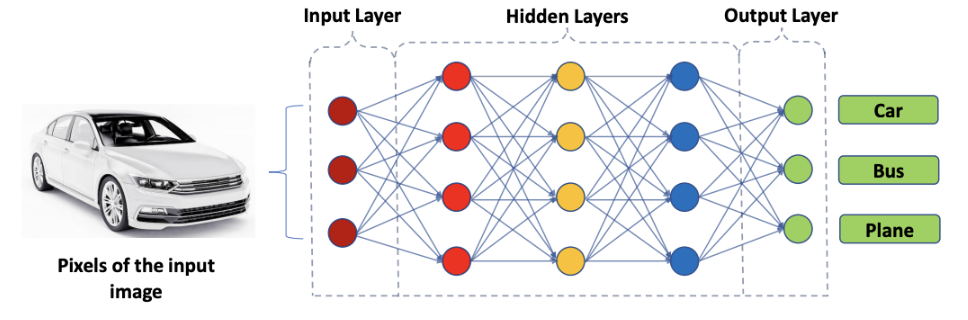
\includegraphics[width=0.6\textwidth]{gambar/cnn.png}
  \caption{Arsitektur CNN \parencite{krichen2023convolutional}.}
  \label{fig:cnn}
\end{figure}

\subsection{\emph{Internet of Things}}
\label{sec:iot}
  
\emph{Internet of Things} (IoT) adalah konsep yang merujuk pada konektivitas jaringan dan kemampuan komputasi yang diperluas ke berbagai objek, perangkat, sensor, dan barang sehari-hari yang tidak secara tradisional dianggap sebagai komputer. Dengan kata lain, IoT memungkinkan perangkat-perangkat ini untuk menghasilkan, bertukar, dan menggunakan data dengan sedikit atau tanpa campur tangan manusia. IoT memungkinkan penggabungan objek fisik ke dalam jaringan digital, sehingga menciptakan ekosistem di mana berbagai perangkat dapat saling berkomunikasi dan bekerja secara otomatis untuk meningkatkan efisiensi dan kenyamanan dalam berbagai aspek kehidupan.

Dalam konteks pertanian modern (\emph{smart agriculture}), IoT telah digunakan untuk meningkatkan efisiensi proses \emph{monitoring} dan aksi otomatis, seperti pengukuran kelembapan tanah, pengendalian irigasi, pelacakan kondisi tanaman, hingga optimasi pemupukan. IoT memberikan keunggulan berupa kemampuan memperoleh data lingkungan secara \emph{real-time} serta memungkinkan pengambilan keputusan berbasis data \parencite{putra2022oil}. Hal ini sangat relevan dalam sistem penyerbukan buatan, di mana data seperti volume \emph{pollen}, status aktuator, dan kondisi perangkat dapat dipantau secara terus-menerus untuk memastikan operasi yang stabil dan konsisten.

\subsection{\emph{You Only Look Once}}
\label{sec:yolo}

\emph{You Only Look Once} (YOLO) merupakan algoritma \emph{deep learning} untuk deteksi objek yang menerapkan pendekatan \emph{single-stage detector}, yaitu menggunakan satu jaringan saraf konvolusional untuk memproses keseluruhan citra secara langsung. Berbeda dengan metode \emph{two-stage detector} seperti \emph{Faster R-CNN} yang memisahkan proses \emph{region proposal} dan klasifikasi, YOLO melakukan prediksi koordinat \emph{bounding box} dan probabilitas kelas secara simultan dalam satu kali inferensi. Pendekatan ini memungkinkan YOLO mencapai kecepatan pemrosesan yang tinggi dengan tetap mempertahankan tingkat akurasi yang kompetitif, sehingga sangat sesuai untuk aplikasi deteksi objek secara \emph{real-time}.

Seiring dengan perkembangannya, YOLO telah mengalami berbagai iterasi mulai dari YOLOv1 hingga versi-versi terbaru yang menawarkan peningkatan signifikan pada aspek akurasi, efisiensi komputasi, dan kemampuan mendeteksi objek berukuran kecil. Setiap versi YOLO memperkenalkan perbaikan pada arsitektur jaringan, mekanisme ekstraksi fitur multi-skala, serta optimalisasi fungsi \emph{loss} untuk meningkatkan performa deteksi. Selain itu, model YOLO modern mendukung konversi ke format ringan seperti ONNX, sehingga memungkinkan implementasi pada perangkat \emph{edge computing} dengan keterbatasan sumber daya. Dalam penelitian ini, YOLO dimanfaatkan untuk mendeteksi objek pada proses penyerbukan kelapa sawit, khususnya bunga betina yang siap diserbuki, sehingga sistem penyerbukan otomatis dapat diarahkan secara lebih presisi \parencite{wang2022yolo}.

\subsection{Raspberry Pi}
\label{sec:raspberry-pi}

\begin{figure}[H]
  \centering
  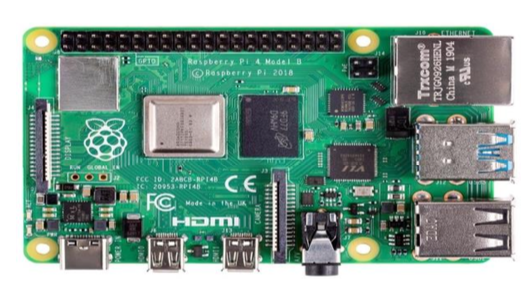
\includegraphics[width=0.6\textwidth]{gambar/raspberry.png}
  \caption{Raspberry Pi Model 4 \parencite{hosny2023internet}.}
  \label{fig:raspberry-pi}
\end{figure}

Raspberry Pi merupakan sebuah komputer berukuran kecil sekelas kartu kredit yang
bersifat open-source dan dikembangkan oleh Raspberry Pi Foundation di Inggris. Perangkat ini
dirancang sebagai komputer berbiaya rendah dengan konsumsi daya yang kecil, namun tetap
mampu menjalankan berbagai tugas komputasi layaknya komputer desktop. Raspberry Pi
memiliki kemampuan pemrosesan paralel karena menggunakan prosesor quad-core, sehingga
cukup andal untuk menangani proses pengolahan data dalam sistem tertanam dan Internet of
Things (IoT). Karakteristik utama seperti portabilitas, biaya murah, fleksibilitas, serta efisiensi
energi menjadikan Raspberry Pi sebagai salah satu platform yang sangat populer dan
menjanjikan untuk pengembangan aplikasi IoT di berbagai bidang \parencite{hosny2023internet}.

Dalam perkembangannya, Raspberry Pi tersedia dalam berbagai model, dengan
Raspberry Pi 5 sebagai versi terbaru saat ini. Raspberry Pi 5 dibekali prosesor 2.4GHz, pilihan
kapasitas RAM yang bervariasi, serta dukungan konektivitas seperti Ethernet, Wi-Fi, dan port
USB yang memadai. Berkat spesifikasi tersebut, Raspberry Pi banyak dimanfaatkan sebagai
pusat pemrosesan data (gateway) dalam sistem IoT, termasuk pada aplikasi transportasi cerdas,
pertanian pintar, dan sistem kesehatan. Kombinasi Raspberry Pi dengan sensor, aktuator, dan
jaringan internet memungkinkan pengumpulan, pengolahan, serta pengiriman data secara real-
time, sehingga mendukung otomatisasi dan pengambilan keputusan yang lebih efektif pada
berbagai sistem cerdas berbasis IoT.

\subsection{\emph{Time of Flight} VL53L0X}
\label{sec:tof}

\begin{figure}[H]
  \centering
  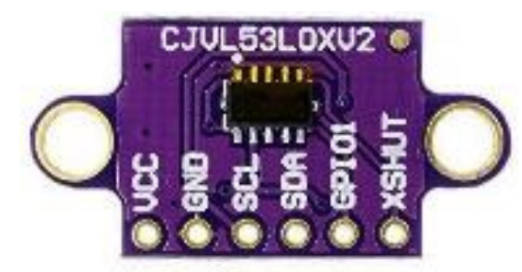
\includegraphics[width=0.6\textwidth]{gambar/tofVL53L0X.png}
  \caption{Sensor \emph{Time of Flight} VL53L0X \parencite{hosny2023internet}.}
  \label{fig:tof}
\end{figure}

Sensor VL53L0X merupakan sensor jarak berbasis Time of Flight (ToF) yang
menggunakan laser inframerah untuk mengukur jarak absolut dengan resolusi milimeter dan
komunikasi I2C. Sensor ini memiliki karakteristik pengukuran yang linear pada jarak dekat
hingga menengah, dengan error yang meningkat pada jarak sangat dekat dan pada permukaan
objek yang sempit atau gelap. Kinerja sensor juga dipengaruhi oleh sudut pancaran dan
penerimaan cahaya, sehingga permukaan objek yang kecil atau tidak rata dapat menyebabkan
ketidakakuratan pengukuran.
Dalam proyek ini, sensor VL53L0X dimanfaatkan untuk mengukur tinggi permukaan
pollen kering di dalam tabung tertutup, di mana nilai jarak hasil pembacaan sensor dikonversi
menjadi volume berdasarkan dimensi tabung. Penerapan pemrosesan data sederhana seperti
moving average digunakan untuk mengurangi noise akibat permukaan pollen yang tidak rata.
Penggunaan sensor pada objek berbentuk tabung dengan permukaan relatif datar diharapkan
dapat menghasilkan pembacaan yang stabil dan konsisten \parencite{hosny2023internet}.

